\chapter{绪论}

\section{课题来源}
红外目标检测是指用红外探测器检测目标与背景之间的红外辐射差异后,对目标进行检测的过程。虽然可见光图像具有图像分辨率高、目标细节完整的特点,但是与红外图像相比容易受到光线变化的影响,大大增加了识别目标的难度。在一些特殊的天气条件下尤其如此,例如下雨天、夜间、有雾天和缺乏可见光源的天气,视距和能见度很低,并且捕获的图像无法正常使用。红外成像技术的特点是工作距离远、抗干扰能力强、测量精度高、受天气影响较小。日夜工作和强大的烟雾穿透能力强使得红外目标检测的市场需求也在不断增加,红外目标检测不仅仅用于军事领域,在工业、安防、交通等民用领域也有广泛的应用,比如红外技术可以应用在无人机上进行全天候的目标检测;在工业界,设备有没有被严重触碰或损坏也可以应用红外技术。尤其是今年疫情期间,红外技术广泛应用于火车站、机场等人流密集的地方,能够实现实时检测体温,避免人工测量体温而造成的拥堵。

本课题主要研究红外图像中的无人机检测算法。本课题来源于哈尔滨海邻科信息技术有限公司“警用人工智能技术合作”。目前,无人机市场发展迅速,为社会带来便利。国外机场无人机干扰航班事件频发,各地无人机“黑航”事件频发。这种现象也受到了部队内外的广泛关注,给机场安全、反恐维稳和国家边境带来了相当大的压力,迫切需要通过对无人机的探测来对无人机施行监控和预警。使用声音、无线电和雷达探测的技术更为常见,但这些技术通常需要昂贵的设备和严格的配置。基于机器视觉的方法具有成本低、配置简单的优点。随着深度学习技术的发展,逐渐应用于各种目标的识别和检测,但是无人机往往在低空飞行,并且还会受到光线和遮挡等因素的影响。检测场景非常复杂,而小尺寸和高速度一直是目标检测的难题。相关监管部门需要利用相关检测网络及时发现管制区域内的非法无人机,以保障人身安全和财产安全。因此,本课题的目的是研究和设计无人机检测算法,以实现快速高效的红外无人机检测。

\section{研究背景与意义}
计算机视觉技术是一种让计算机从给定的图像或视频中获取相关信息并进行“感知”的技术,是人类视觉感知的扩展。半导体行业促进了硬件水平的提高,也带动了机器视觉的发展,使其在人工智能领域得到广泛应用。

随着各方面技术的成熟,研究人员在不断提高红外探测系统的性能。红外探测技术广泛应用于军事领域,如红外预警、水下搜索和红外导航中,还应用于医疗损伤、细胞诊断、工业探伤等民用领域,在军事和包括医疗在内的民用领域取得突出成就。
自1960年代初以来,红外热成像已经开始用于医学\cite{ring1975thermography}。早期的成像系统很大,显示和测量温度的设施非常有限
。在 1970 年代,热像图的计算机图像处理投入使用,增加了对图像进行定量和存档的可能性。如在疾病诊断和预防领域,大多数风湿性疾病的共同因素是关节炎。 辐射测量和热成像已被证明可以指示和测量由局部炎症引起的发热。 在类风湿性关节炎、幼年型关节炎、骨关节病、痛风和强直性脊柱炎中,受累关节的热量分布异常。 实验数据表明,温度变化反映了关节的炎症状态,这一结论可用于衡量口服、全身和局部药物治疗以及手术(即滑膜切除术)的治疗效果。

在计算机视觉领域中,当前主流的探测系统可分为3类:可见光探测、红外成像探测和雷达探测系统,基于红外探测系统的红外弱小目标检测一直都是一个重要的课题和研究热点。红外探测系统主要对对目标的温度与本身的材料特性敏感,而与环境等因素相关性较小,使得其在3类探测系统中脱颖而出,具有一系列优势:
(1)不受光照的影响,可以全天时工作;
(2)由于其不发射电磁波,因此是非主动的探测方法;
(3)穿透能力强,可以避免灰尘、云层和烟雾等的遮挡,可以更好地识别虚假的伪装目标。以上优势也使其成为传统可见光探测系统与雷达探测系统的有效补充或替代。

实时检测红外目标,高检出率、低误报率是实际应用中重要的要求。一般情况下,待检测目标与检测器之间的距离较长,因此,红外目标在整个红外图像中占据的区域非常小。它们通常小于 100 像素,背景复杂、易变且难以检测。具体表现如下:

(1)红外目标的特点:弱小红外目标缺乏颜色、纹理等属性,尺寸较小。 (通常小于 9×9 像素)大多数方法仅适用于灰度分布特征、运动属性和运动方向等特征。此外,小型红外目标的信噪比较低。并且经常被复杂而动态的背景所掩盖,还会受到云层和海浪的干扰。

(2) 红外背景的特点:背景相似,分布连续。目标通常在云和波浪中。场景复杂多变。复杂红外图像的背景特征有些不均匀,并且相对灰度比目标区域低。

(3) 红外目标检测中的困难: 1) 目标的可用特征较少。因为目标很小,所以总辐射能量小于背景辐射能量。图像中的灰度分布是可变的,很难使用统一的数学模型来描述,而且它缺乏传统可见光目标的纹理、形状和其他结构信息。传统可见光检测方法不能用于检测小而弱的红外目标,或是一般性能较差。 2)图像的信噪比低。由于成像距离远,小目标难以和杂波和噪声区分开,容易被淹没在云层和海浪中,使得检测算法容易受到干扰。 3)检测精度往往不高。在实际情况和使用中,目标的运动方向和速度具有很强的机动性。这使得提高机动目标的检测精度成为学术界致力于解决的问题。4)成像环境复杂。在特种成像方面,成像过程往往伴随着烟雾和海浪。这导致对不同检测算法的鲁棒性提出更高的要求。 5)实时性较差。检测效果通常与计算量成近似反比。检测效果好的算法往往需要大量的计算。因为建模体积大、硬件处理能力不足,常常导致实时性能不佳。6)很少有公开数据集。红外目标检测主要用于军事领域,具有一定的保密性。可供研究人员公开使用的红外数据集很少,这在一定程度上限制了红外目标检测算法的发展。本课题检测的目标图像如图\ref{uav}所示。

\begin{figure}[htbp]
    \centering
    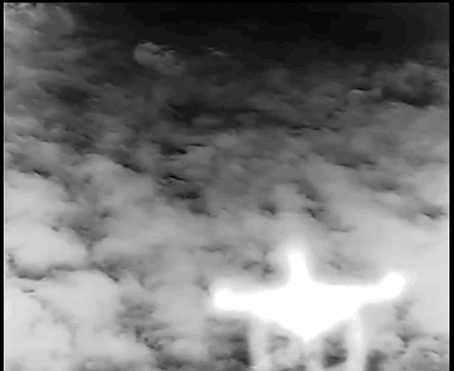
\includegraphics[width = 0.8\textwidth]{无人机目标示例.png}
    \caption{无人机目标示意图}
    \label{uav}
\end{figure}

综上所述,红外图像的无人机目标检测应用广泛,研究价值很大。本文基于深度学习算法,针对红外无人机目标进行研究,针对红外图像无人机目标检测的特点,从数据增强、网络结构改进、网络轻量化、嵌入式实现这四个方面展开研究。

\section{国内外研究发展现状}
目标检测算法一般包括分类和定位两个子任务,常用于检测图像中某些已知类别的对象。本节主要从传统的目标检测算法、基于深度学习的两阶段目标检测算法、基于深度学习的单阶段目标检测算法以及针对红外图像的目标检测算法4个方面来介绍本文研究领域目标检测算法的研究现状\cite{尹宏鹏2016基于视觉的目标检测与跟踪综述}。

\subsection{传统的目标检测算法}
如图\ref{ct}所示,传统的目标检测算法流程是首先通过某种算法得到选定的待检测区域,对该区域经过特征提取,最后输入分类器进行分类后得到检测结果。

\begin{figure}[htbp]
    \centering
    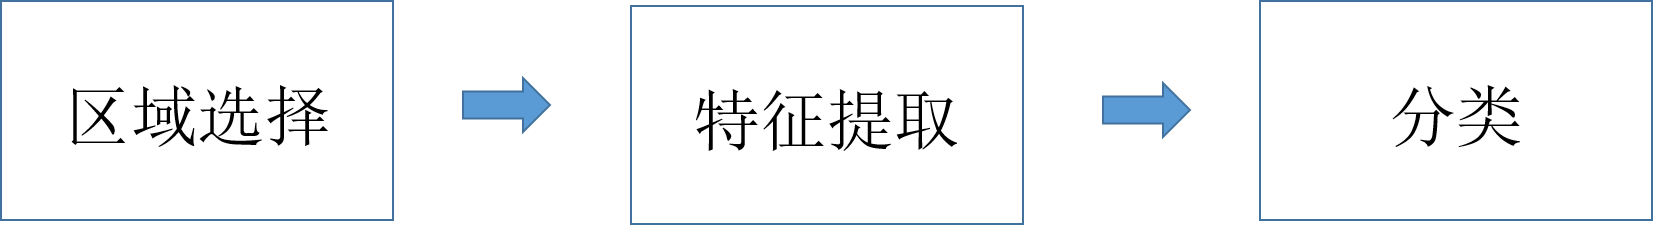
\includegraphics[width = 0.6\textwidth]{传统目标检测.png}
    \caption{传统目标检测流程}
    \label{ct}
\end{figure}

传统的目标检测算法在进行计算时,对于初始区域的选择是使用遍历的方式搜索整个图像的不同比例纵横比的滑动窗口,得出候选区域,即某个可能包含目标的区域\cite{胡伏原2020基于卷积神经网络的目标检测算法综述,kira1992feature}。这种暴力穷举法的特点是时间复杂度很高,而且会产生大量的重复窗口,不仅影响后续的特征提取的准确性,而且会拖慢整个算法的运行时间。后来研究人员设计了效率更高的区域选择算法,比如有选择性搜索算法(Selective Search)\cite{uijlings2013selective}以及Edge Boxes算法\cite{zitnick2014edge}等。选择性搜索算法首先将原始图像划分为多个尺寸较小区域,然后根据计算出的某两个区域之间的相似度和这两个区域的大小依次组合相邻的小区域,反复执行上述过程,直到在整幅图像内组合成一个大区域。Edge Boxes算法则是充分利用若干个edge box相互之间潜在的相似性,根据权重的值来确定某个box中包含的轮廓的数量或与该box的边界产生重叠的轮廓的数量,之后根据上述统计信息对每个box进行打分和评估,确定出候选box。之后的第二步是从候选区域中通过特定的特征提取算法提取特定长度的特征向量,以获得该区域的语义信息,做出对目标分类的预测。一般情况下,包括在目标检测领域中,传统机器学习算法会选择向机器学习模型中输入工艺特征。然而,由于物体的形状和尺寸多变、光照会随时间和天气不断变化、背景的多样性,设计一种鲁棒的特征提取算法往往比较困难,而提取特征模块的性能好坏直接影响到后续的分类模块的准确性。在特征提取的阶段,HOG函数\cite{he1990texture}和SIFT函数\cite{lowe1999object}是较为常用的特征表达函数。HOG算法首先会将图像分割成一些小的连通区域(细胞单元),之后在每个单元处对每个像素点的梯度直方图进行采样,或是对单元边缘区域的梯度直方图进行采集,HOG算法将用这种方式获取的直方图称作该单元的特征。与其他的特征描述方法相比,HOG有很多优点。首先,由于HOG是在图像的局部方格单元上操作,所以它对图像几何的和光学的形变都能保持很好的不变性,这两种形变只会出现在更大的空间领域上。其次,在粗的空域抽样、精细的方向抽样以及较强的局部光学归一化等条件下,只要行人大体上能够保持直立的姿势,可以容许行人有一些细微的肢体动作,这些细微的动作可以被忽略而不影响检测效果。
因此HOG特征比较适合用于图像中的人体检测任务。SIFT算法的处理方法是首先计算出输入图像的DoG尺度空间,之后在该DoG空间中求出极值点,然后调整尺度空间DoG函数,拟合出近似的DoG函数,以准确找到关键点,并去除不稳定的关键点。然后计算剩余关键点的主要方向用以创建 SIFT 描述子。SIFT函数的特点是具有尺度不变性和旋转不变性,此外还具备适应复杂光照背景变化的能力,因此在传统目标检测算法中得到广泛应用。

在完成对图像特征的提取之后,算法将使用分类器对待测目标进行分类。
分类器相关算法主要有Adaboost\cite{freund1997decision} 算法等,而经典的分类器主要有SVM\cite{cortes1995support}分类器等。
常用于对分类器进行优化的AdaBoost算法属于一种常见的Boosting算法。
Boosting, 也称为增强学习或提升法,是⼀种重要的集成学习技术,能够将预测精度仅⽐随机猜度略⾼的弱学习器增强为预测精度⾼的
强学习器,这在直接构造强学习器⾮常困难的情况下,为学习算法的设计提供了⼀种有效的新思路和新⽅法。其中最为成功的应⽤就是AdaBoost算法。
AdaBoost是英⽂"Adaptive Boosting"(⾃适应增强)的缩写,它的⾃适应在于:前⼀个基本分类器被错误分类的样本的权值会增
⼤,⽽正确分类的样本的权值会减⼩,并再次⽤来训练下⼀个基本分类器。同时,在每⼀轮迭代中,加⼊⼀个新的弱分类器,直到达到某个
预定的⾜够⼩的错误率或达到预先指定的最⼤迭代次数才确定最终的强分类器。
Adaboost算法的流程可以简述为三个步骤:

 (1)⾸先,初始化训练数据的权值分布。假设有$N$个训练样本数据,则每⼀个训练样本最开始时,都被赋予相同的权值。

 (2)然后,训练弱分类器。具体训练过程是:如果某个训练样本点,被弱分类器准确地分类,那么在构造下⼀个训练集中,它对应
的权值要减⼩;相反,如果某个训练样本点被错误分类,那么它的权值就应该增⼤。权值更新过的样本集被⽤于训练下⼀个分类器,整个训
练过程如此迭代地进⾏下去。

 (3)最后,将各个训练得到的弱分类器组合成⼀个强分类器。各个弱分类器的训练过程结束后,加⼤分类误差率⼩的弱分类器的权重,使
其在最终的分类函数中起着较⼤的决定作⽤,⽽降低分类误差率⼤的弱分类器的权重,使其在最终的分类函数中起着较⼩的决定作⽤。误差率低的弱分类器在最终分类器中占的权重较⼤,否则较⼩。

支持向量机(support vector machines, SVM)是一种二分类模型,它的基本模型是定义在特征空间上的间隔最大的线性分类器,间隔最大使它有别于感知机;支持向量机还包括核技巧,这使它成为实质上的非线性分类器。支持向量机的学习策略就是间隔最大化,可形式化为一个求解凸二次规划的问题,也等价于正则化的合页损失函数的最小化问题。支持向量机的学习算法就是求解凸二次规划的最优化算法。

传统的机器学习算法对于目标检测问题能取得一定的检测效果,但是对于复杂任务还是存在性能瓶颈。分析其算法原理可以发现传统的目标检测算法都存在两个问题:

(1)算法的复杂度高,在整体流程较为冗长、步骤较多的同时,各个部分单独的时间复杂度也较高,因此整体效率往往较低。具体到区域选择算法中,虽然区域选择算法从原始的滑动窗口算法到选择性搜索算法已经有了较大的效率提升,但是仍然存在选择过程没有针对性的固有问题,结果中仍然会保留相当数量的多余窗口,会影响到后续的分类模块的检测精度和速度。

(2)手工设计的特征往往带有一定的特殊性,因此对于目标检测任务的多样性往往难以匹配足够的泛化能力,在背景和目标尺度等条件变化较大时,手工设计的特征难以适应这些变化,往往无法准确地获取目标的语义信息,因此检测的精度会产生较大波动,总体精度不高。

因此区别于传统的目标检测算法的流程冗长和可学习特征量不足等问题,深度卷积神经网络能较好地部署端到端的系统算法,能从整个流程上优化算法的运行效率。此外,深度卷积神经网络能容纳更多的模块和参数,也就是能拟合更加复杂的目标函数,在充分训练之后,深度神经网络对输入信息的捕捉和表达能力更强。并且随着相关研究的持续进行,深度卷积神经网络可以将网络分成各类具有特殊功能的模块,比如可以将位置信息和语义分类信息通过不同的网络层进行提取和增强。正是因为基于深度学习的目标检测算法相对于传统机器学习检测方法有很多显著的性能优势,同时随着计算机计算能力的快速发展,基于深度学习的目标检测算法成为了重点研究领域,研究人员不断设计各种新算法,不断在目标检测任务中取得更好的性能。

\subsection{基于深度学习的两阶段目标检测算法}
两阶段目标检测算法也称为基于候选框的目标检测算法。这种目标检测算法主要分两步进行:

(1)通过对输入图像的计算,应用特定算法得出若干候选区域。这一步骤中经常使用的算法有选择性搜索和Edge Boxes等。

(2)对候选区域应用卷积神经网络(Convolutional Neural Networks, CNN)进行推理,卷积神经网络主要用于特征的提取和得出分类结果。

2014 年,Girshick 等人开创性地提出不再使用传统的
滑动窗口+手工特征的目标检测方法,而是使用选择性搜索+卷积神经网络进行代替。经过研究后提出了 R-CNN 模型框架\cite{girshick2014rich},经过实验,证明了卷积神经网络相比于传统的 HOG
等手工特征在 PASCAL VOC 2007数据集上的目标检测性能更好,进一步说明了深度学习算法
在目标检测领域的有效性和优越性,以该算法为起点,掀起了一波研究基于深度学习的目标检测算法的风潮。如图
\ref{rcnn}所示,R-CNN算法的流程主要由 4 个步骤组成:

\begin{figure}[htbp]
    \centering
    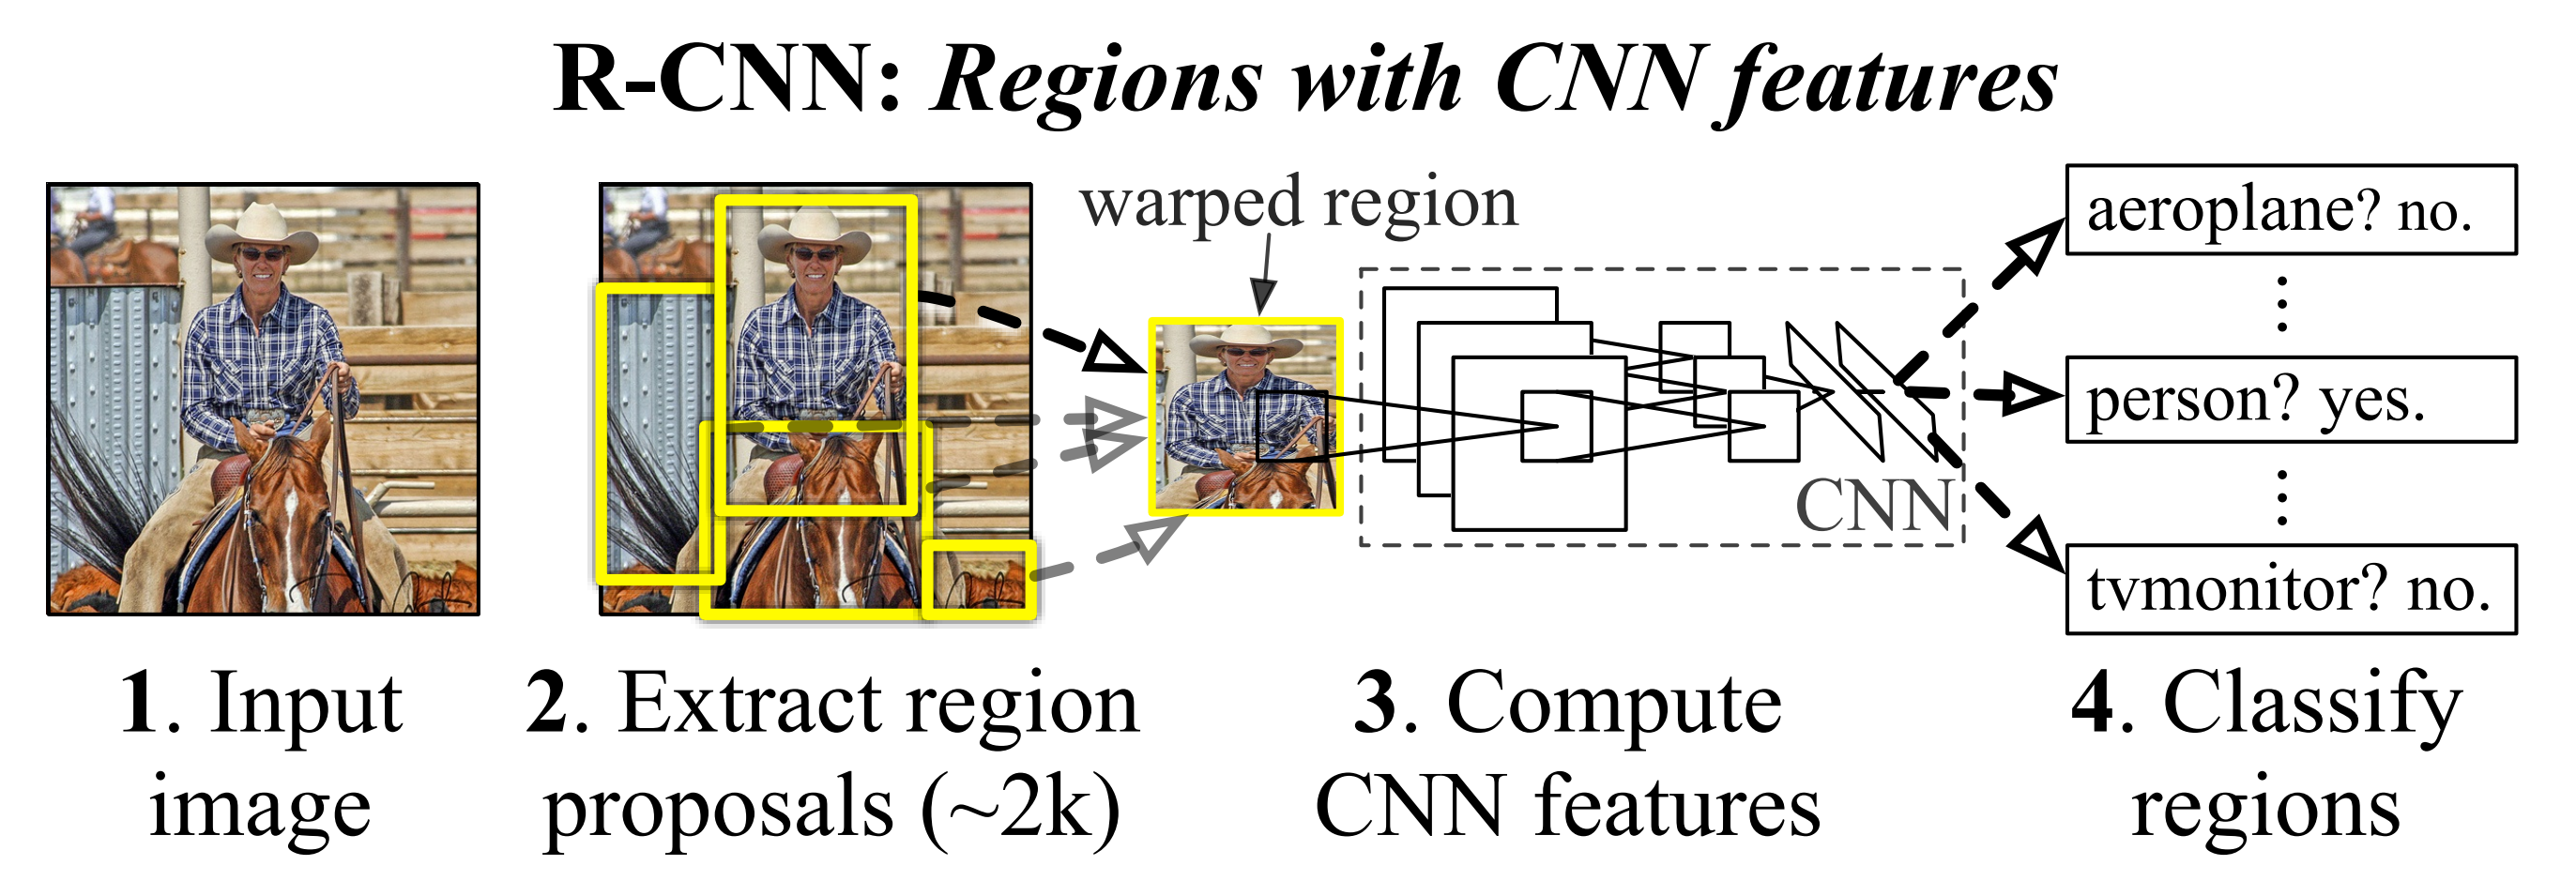
\includegraphics[width = 0.7\textwidth]{rcnn.png}
    \caption{R-CNN算法框架}
    \label{rcnn}
\end{figure}

(1)对于每张输入图片,通过选择性搜索
算法产生 $1000\thicksim2000$个候选区域,把这些区域经过缩放后调整到后续网络需要的大小。

(2)对每个候选区域分别使用卷积神经网络提取目标的特征,将提取的特征以特征向量的形式输出。

(3)在接收到前序模块输出的特征向量作为输入后,支持向量机分类器进行分类,对于每个类别分别训练各自的分类器,各个分类器之间相互独立,不共享参数。

(4)因为候选框是经过不完善的选择型搜索算法计算得出,因此需要对候选框位置进行适当修正,这一过程一般情况下使用 bounding-box 回归器。

经过分析算法原理可知,相比于传统的目标检测算法,卷积神经网络的特点是能在不同层网络捕捉到特定目标的待求尺
寸信息,并且经过计算可以生成的feature map能够充分表征目标的各种特征。R-CNN模型对 AlexNet 网
络结构进行了应用,此外还借鉴并优化了 fine-tuning方法。经过在 PASCAL VOC 2007 数据集上的实验证明,准确率可以达到 58$\%$,而使用 VGG16 网络结构的版本在 PASCAL VOC 2007 数据集上的准确率达到 66$\%$,这个结果
和传统算法相比高了约 20$\%$。

但是R-CNN算法并不完美,主要有以下3个问题:

(1)整个算法网络结构训练需要分为好几个阶段,训练时间长,步骤繁琐的同时容易产生错误。

(2)区域选择算法的效率仍然存在改进空间。选择性搜索算法会导致每张图片提取到过多的候选区域,存在较多冗余候选区域,常常增加训练耗时,大大影响算法的整体效率。并且选择性搜索算法的鲁棒性有限,很难保证在复杂背景下选择出高质量的候选框。

(3)候选区域提取算法不仅仅会产生大量冗余的候选框,这些提取到的候选框是分别进入到卷积神经网络中进行特征提取,因此除非对算法进行特别设计的并行优化,该算法无法避免地会产生大量重复的无用计算,大大降低算法的时间效率。

之后何凯明等人经过研究空间金字塔匹配(SPM)概念,特别针对 R-CNN 在
提取特征时存在重复计算等问题,提出了创新的SPP-Net\cite{purkait2017spp},有效地解决了R-CNN 对所有的候选
区域全部无选择地输入网络提取特征的问题。主要方法是对整张图片一次性地利用卷积神经网络提取特征,
并将提取到的特征通过 SPP 转变成固定长度的特征向量,之后将特征向量输入到全连接层。这样就实现了加快
R-CNN 的目标,同时还减少了算法的计算量。SPP的流程不经过原来R-CNN 中输出固定大小候选区域的处理步骤,因此也不会引起信息的丢失和引发几何失真等问题。但
SPP-Net仍然存在局限性。SPP-Net不能使用梯度反传算法(BP)对某些层的参数进行更新,
并且SPP-Net的训练仍然是多阶段过程。此后,经过研究SPP-Net 的两个局限点后,2015 年 Girshick 提
出的 Fast R-CNN\cite{girshick2015fast}算法首创性地将SPP-Net 和 R-CNN 的优点进行结合,不仅提取特征的方式改进成一次性地将整张图像输入到网
络中进行,还应用了多任务损失函数(主要是分类和回归等),最终结果是整个训练过程除
了提取候选区域以外的过程都实现了端到端优化,这一改进也大幅优化了 R-CNN 中存在的多阶段训练和
存储而消耗大量时间和存储资源的问题。该算法的创新点有:

(1)和以往的R-CNN算法不同,Fast R-CNN开创性地将分类损失函数和回归损失函数融合起来组成一种新的复合损失函数,
统一进行网络的训练。

(2)使用 softmax 取代原来的支持向量机分类器。

(2)设计使用ROI池化模块。ROI
池化层是一种相比 SPP-Net 空间金字塔池化层更简洁的池化层模块,主要作用是能将图像
应用候选框选择算法计算得出的候选框添加到最后一个卷积层输出的 feature map 上,
之后经过 ROI池化输出固定大小(一般所使用的为最大池化)。经过实验,Fast R-CNN算法在
PASCAL VOC 2007 数据集上的mAP 可以达到 66.9$\%$,虽然相比于 R-CNN 仅仅提升了 0.9
个百分点,但是Fast R-CNN的训练速度达到了R-CNN算法的 9 倍。

Fast R-CNN算法仍然存在问题。该算法的局限性主要是仍然没有拜托相对低效的区域选择算法,Fast R-CNN使用的选择性搜索或 Edge Boxes 算法主要基于相对固定的低级视觉信息,也就是无法通过数据驱动方式进行学习和进化,并
且时间效率较低。Fast R-CNN算法的主要框架如图\ref{fastr}所示。

\begin{figure}[htbp]
    \centering
    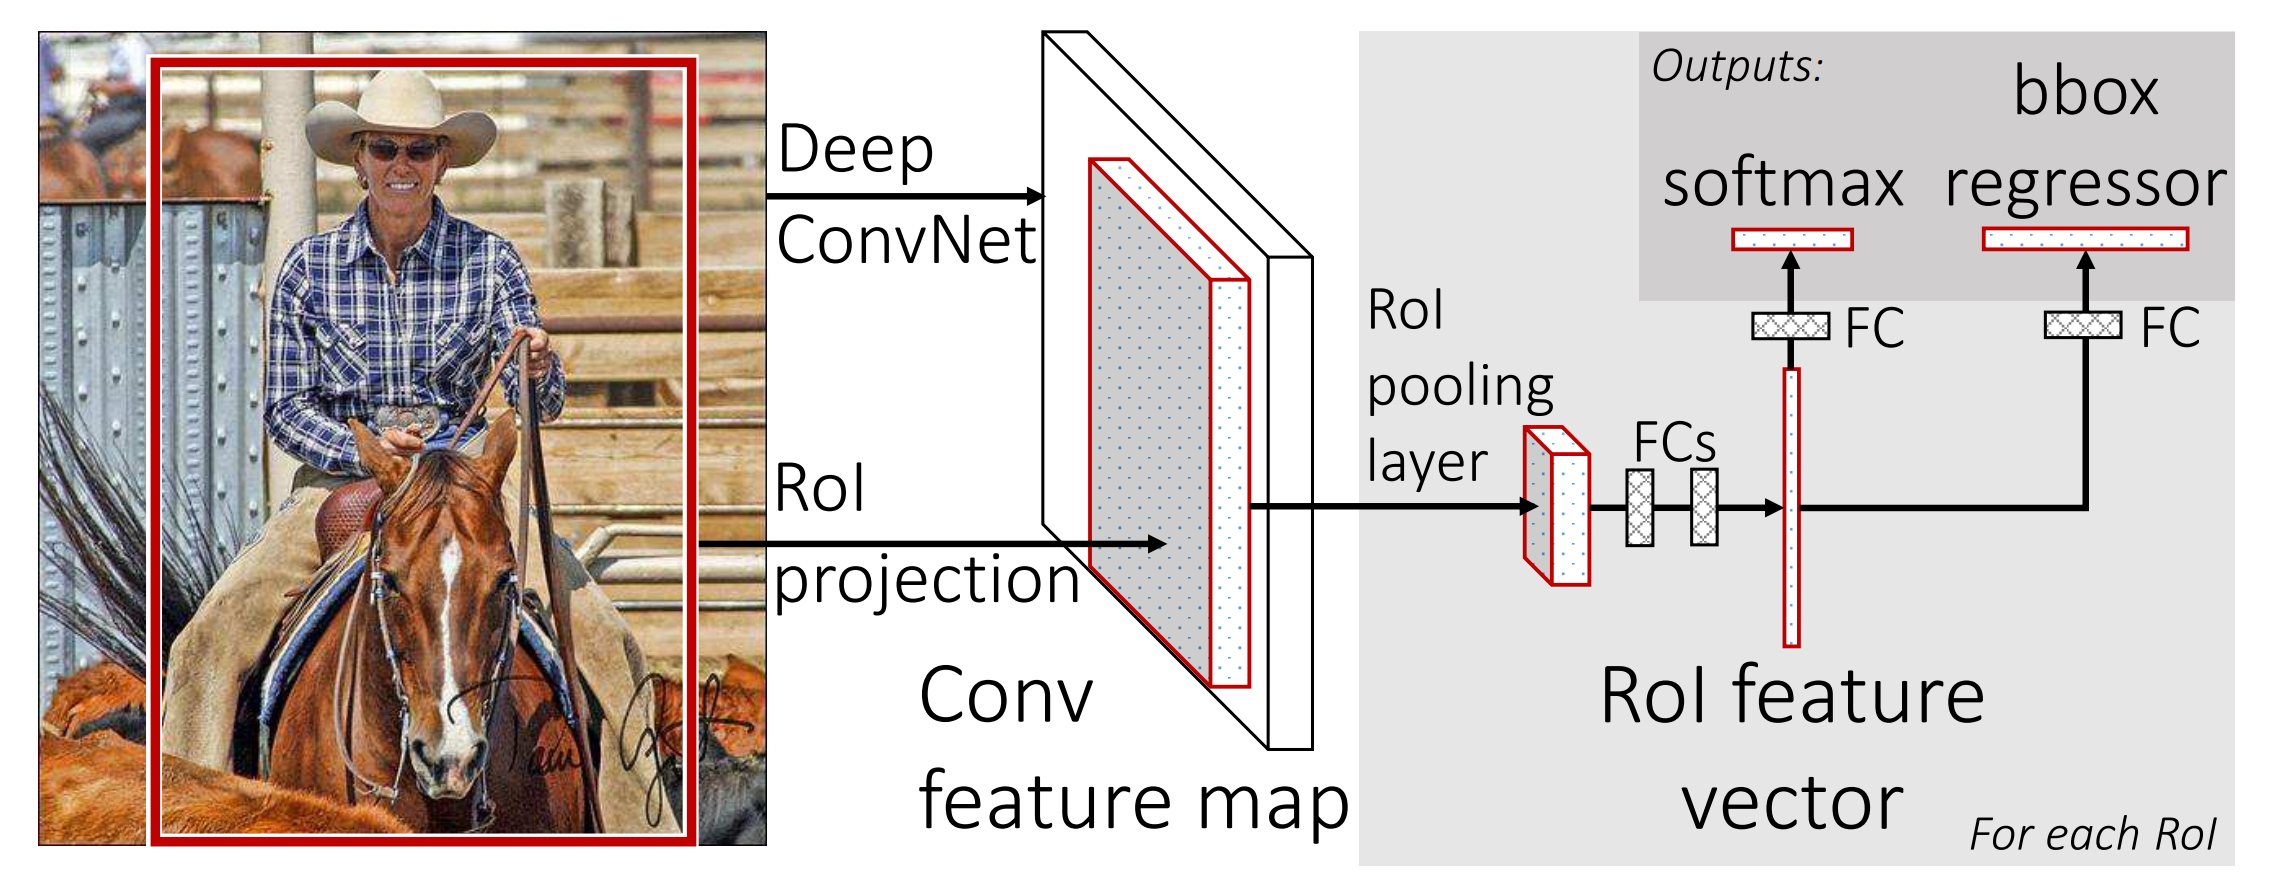
\includegraphics[width = 0.9\textwidth]{fastr.png}
    \caption{Fast R-CNN算法框架}
    \label{fastr}
\end{figure}

2016 年,Ren 等人针对 R-CNN系列算法的候选区域算法普遍存在的候选区域提取速度的问题,研究并提出了 Faster R-CNN 算法
\cite{ren2015faster},Faster R-CNN 算法的主要框架如图\ref{fasterr}所示。

\begin{figure}[htbp]
    \centering
    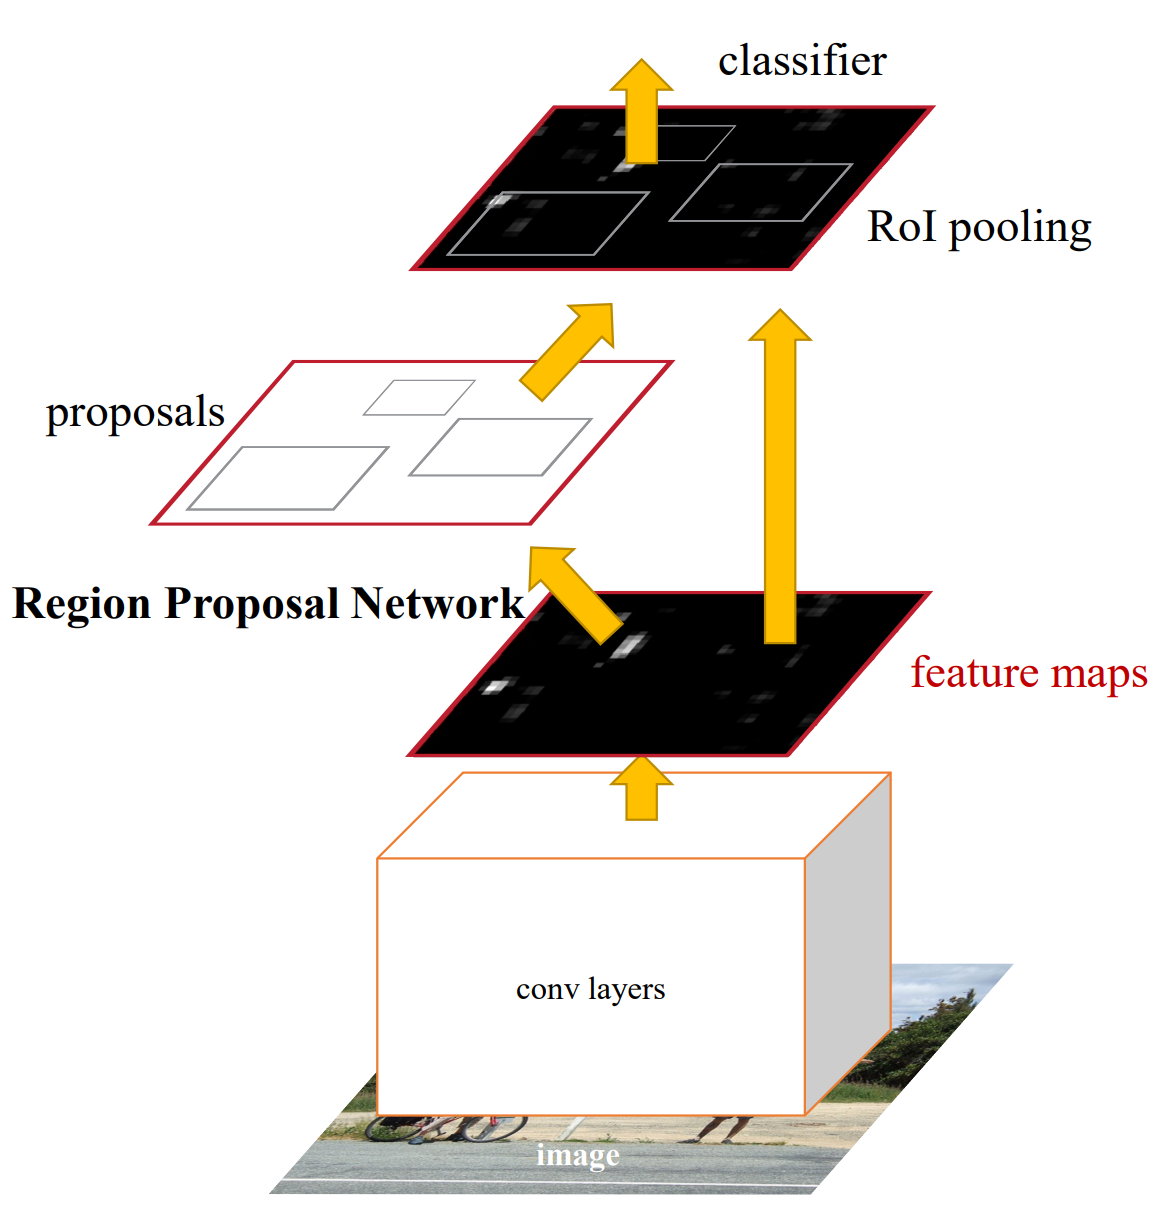
\includegraphics[width = 0.7\textwidth]{fasterr.png}
    \caption{Faster R-CNN算法框架}
    \label{fasterr}
\end{figure}

Faster R-CNN 算法的主要贡献是创新地使用 Region
Proposal Network(RPN)网络替代选择性搜索算法,由于 RPN 与检测网络主体
共享全部的卷积特征并且还有一组公共的卷积层,因此可以实现算法网络的端到端训
练。Faster R-CNN 算法的实现过程是:

(1)将输入图像输入VGG-16网络进行特征的提取。

(2)使用 RPN 生成proposals。RPN 是一种全卷积网络,能够通过 $n \times n$ 的滑动窗口在特征
图上逐点滑动,在特征图的每个位置上以窗口为中心用 9 种(三种尺度,三种长宽比)
anchor 生成 proposals,然后对每个 proposal 进行判断,判定其是否为背景,并进行初步的回归。

(3)将 RPN 得到的的输出作为输入送进Fast R-CNN,通过 ROI池化输出固定大小 feature map 后进行更为精细的分类工作,此外对检测框的位置进行进一步修正。

Faster R-CNN 的NIPS2015 版本使
用的主要框架是 RPN+Fast R-CNN 网络,整体流程跟 Fast R-CNN一样。经过实验,该算法在 PASCAL VOC 2012 数据集上的mAP 可以达到73.2$\%$,此外该算法具备比Fast R-CNN快10倍的运行速度。

Faster R-CNN 算法的局限主要集中在以 ROI 池化层为界,网络的功能较为固定,前面一部分子网络用于特征提取,后面
一部分子网络用于目标检测,并且在对候选框分类和回归任务需要分别在全卷
积网络中进行各自的计算,因此算法整体的计算量仍然很大,该算法仍然在多数情况下达不到实时检测的要求,并且对小尺寸目标的检测效果比较差。

通过研究人员的不懈努力,基于候选框的目标检测算法在 Faster R-CNN 之后仍然在不断进步,目前具
有代表性的主要有 R-FCN\cite{dai2016r}和 Mask R-CNN\cite{he2017mask}。Faster R-CNN 的问题在于虽然初步实现了网络的端到
端训练,但是整个网络以 ROI 池化层为界前面是共享全卷积网络,后面是分类网络,不能达到共享计算的效果,因此整个算
法运行的时间效率较低。而经过理论研究,算法所使用网络的backbone卷积层数越深,就能获得有意义的语义特征,进而更加有利于最终的分类任务的正确完成。但是与此同时,网络层数加深会导致目标的位置信息丢失
,最终会使得算法对待测目标的定位能力受损。

由于目标检测的任务是对图像中的待测目标进行位置和分类的求解,通过对ResNet、GoogLeNet
提出的分类网络和检测网络的平
衡问题进行研究与分析,R-FCN 提出了一种position-sensitive score mAP的概念。R-FCN 的backbone采用ResNet-101(去
掉最后一层 FC 层),将conv4层的输出作为 RPN 的输入,计算得到ROI,之后将网络
最后输出的 feature map用来计算position-sensitive score mAP,分别进行回归和分
类。经过实验证明,R-FCN可以在不损失精度的情况下获得比 Faster R-CNN大2.5 倍的运行速度。算法框架如图\ref{rfcn}所示。

\begin{figure}[htbp]
    \centering
    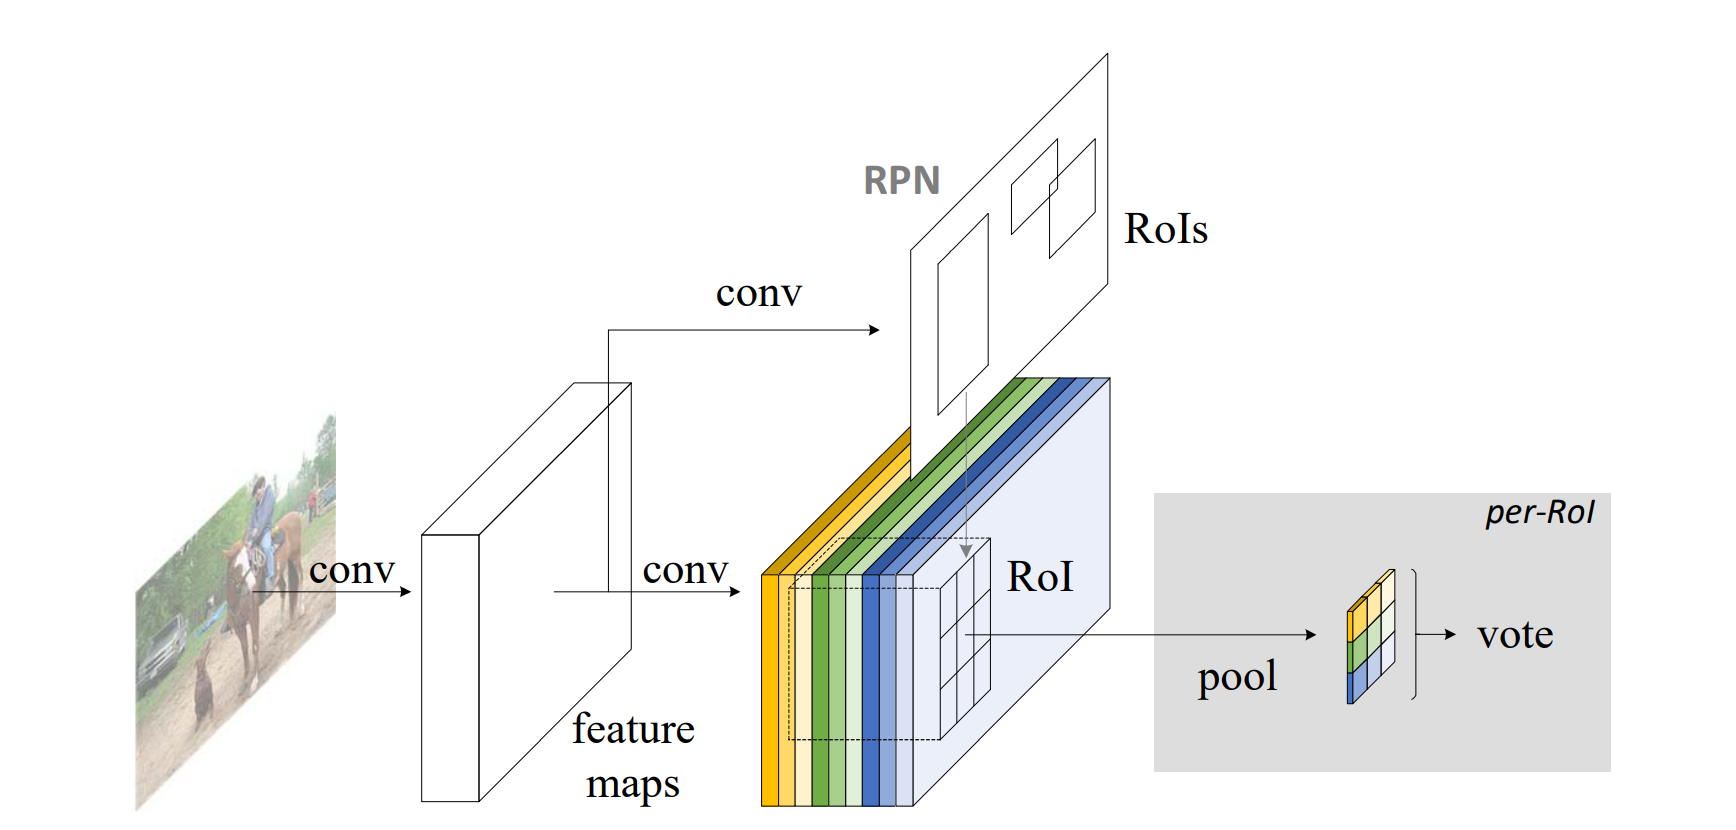
\includegraphics[width = 0.9\textwidth]{rfcn.png}
    \caption{R-FCN算法框架}
    \label{rfcn}
\end{figure}

Mask R-CNN 是以 Faster R-CNN 为原型,增加了一个 mask 分支
用于实例分割任务,此网络最大的创新点在于 ROI Align 的提出,解决了目标映
射到 feature map 上可能会出现坐标不是整数问题。ROI 池化 层需要输出固定
大小的 feature map 而进行等比例缩放过程中引入了量化误差,虽然量化只是去
掉了小数部分,但是映射到原图上误差会成倍的增长,从而严重影响网络的定位
准确性。在 ROI Align 中提出了双线性插值填补非整数位置的像素,使用 max 或
average 池化 汇总结果,整个过程没有使用量化,从而获得更准确的像素信息,
进一步提高了检测的精度,算法框架如图\ref{maskr}所示。

\begin{figure}[htbp]
    \centering
    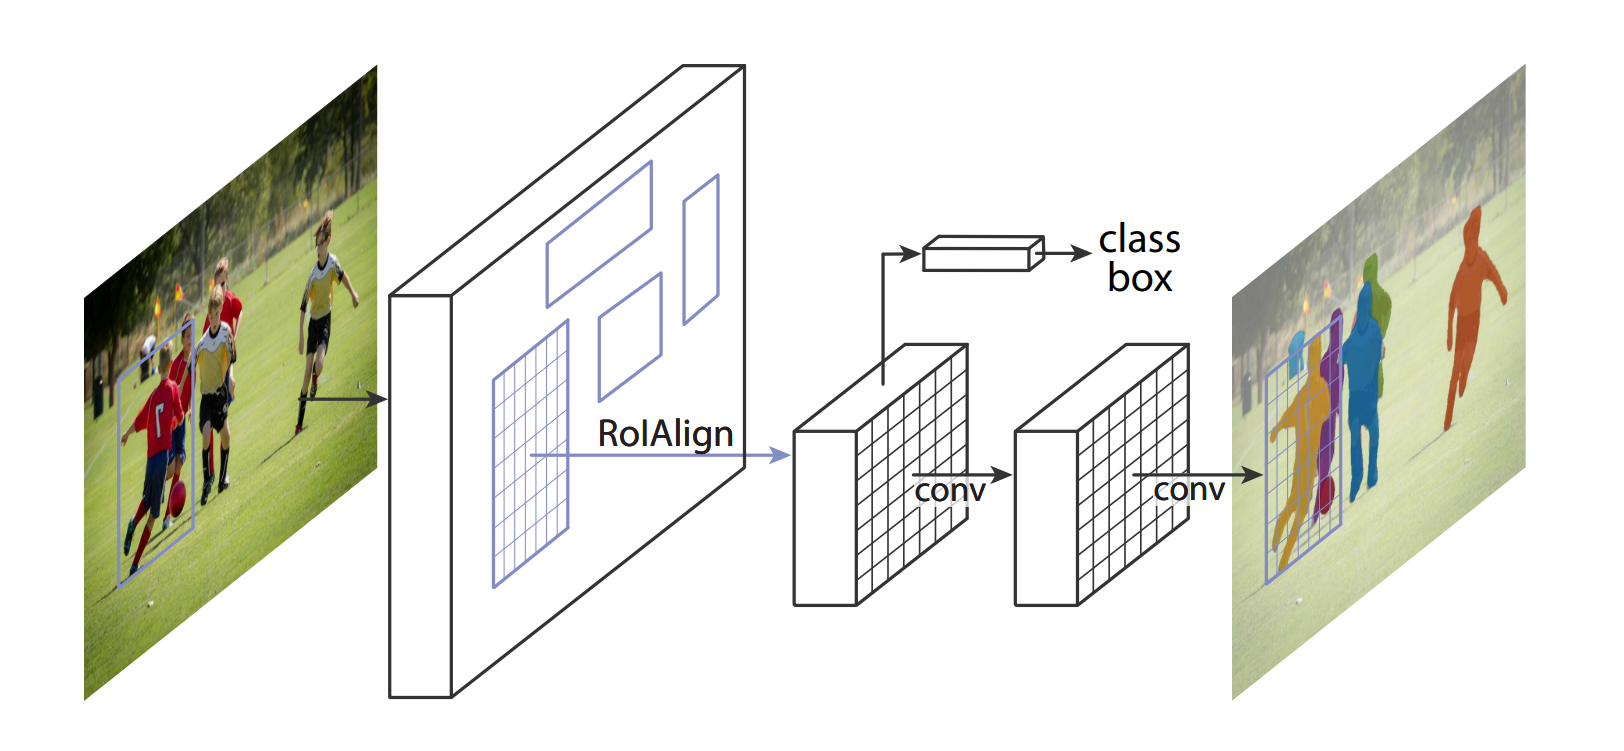
\includegraphics[width = 0.9\textwidth]{maskr.png}
    \caption{Mask R-CNN算法框架}
    \label{maskr}
\end{figure}

\subsection{基于深度学习的one-stage目标检测算法}
基于候选框的目标检测算法速度提升的关键是将目标检测问题转化为多区
域分类问题,充分利用目标在整个图片的上下文信息。对此,研究者们提出了一
种速度比基于候选框的目标检测算法快很多的基于回归的目标检测算法,基于回
归的目标检测算法没有候选框生成阶段,而是将图像上所有位置都视为潜在对象
去尝试对每个感兴趣的区域进行分类\cite{jiao2019survey,wu2020recent}。
2016 年 Redmon 等人提出的 YOLO(You Only Look Once)将目标检测看作
是回归问题\cite{redmon2016you},整个框架将目标分类和定位通过一个单一的网络完成,省略了候
选框生成步骤。YOLO 框架为图\ref{yk}所示,YOLO 直接在输出层回归 bounding box
的位置和所属类别,从而实现 one-stage。YOLO 的目标检测流程为:

\begin{figure}[htbp]
    \centering
    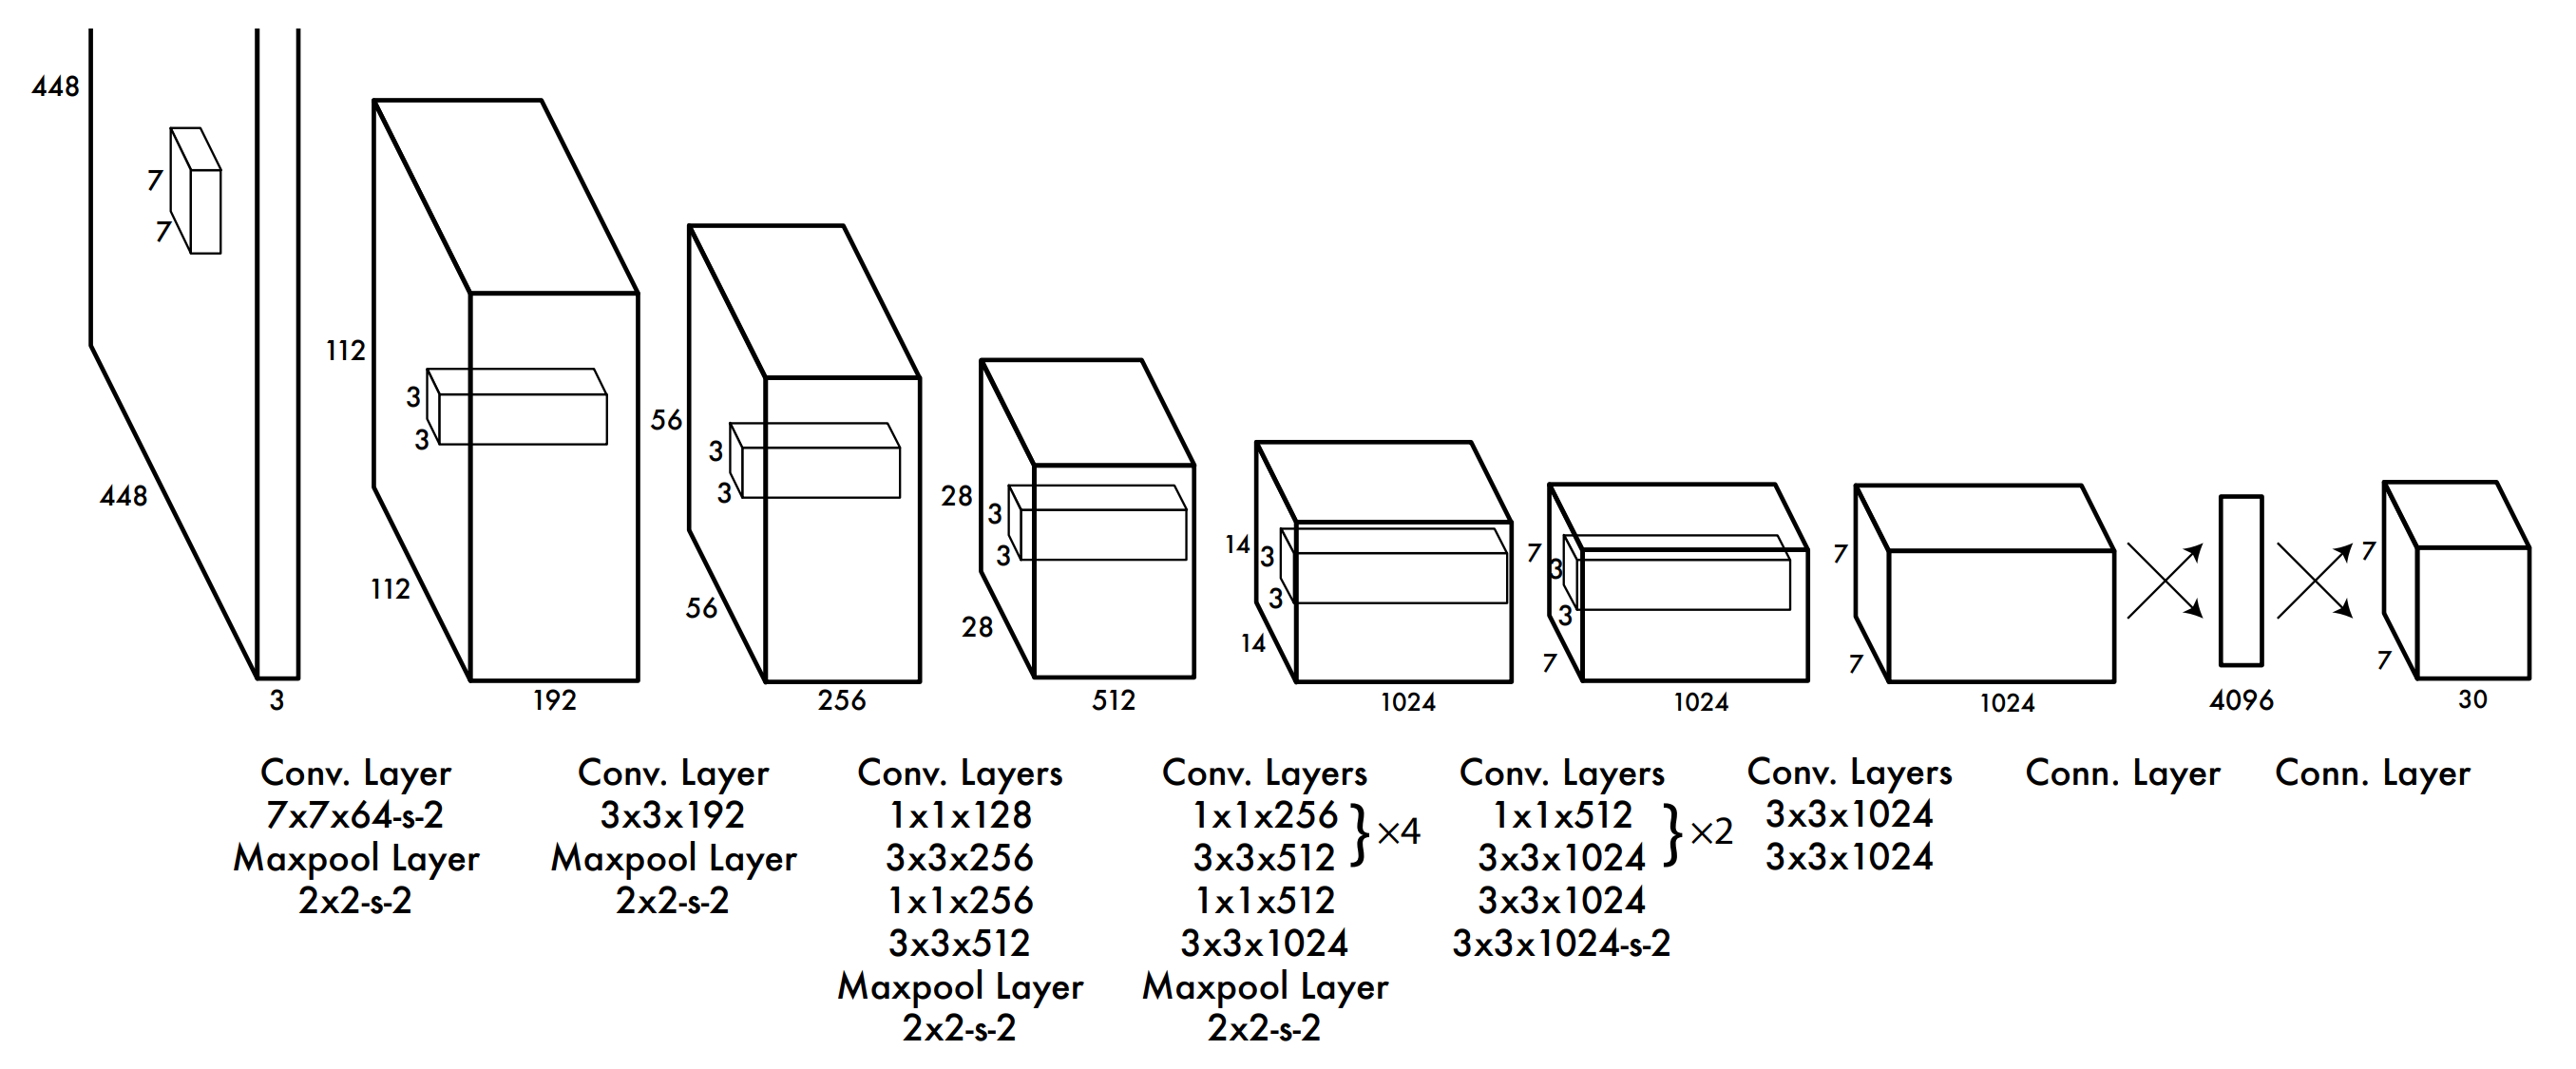
\includegraphics[width = 0.9\textwidth]{yolo框架.png}
    \caption{YOLO算法框架}
    \label{yk}
\end{figure}

(1)将输
入的图像划成 $7 \times 7$ 个网格;

(2)对每个网格预测两个 bounding boxes(每个
bounding box 包含五个参数(x,y,w,h,confidence)以及类别概率);

(3)对最后
输出的 $7 \times 7 \times 2$ 个预测窗口设置阈值用 NMS 去掉可能性低的窗口。这样设计网络
在候选框处理过程中节省了时间,加快了网络的推理速度,经过测试 YOLO 可
以达到每秒 45FPS 的检测速度,能够达到实时性的要求。

YOLO 算法的局限性在于:

(1)要求输入图片的尺寸固定($448 \times 448$)

(2)
由于在每个网格上只能预测两个 bounding boxes,难以检测到小目标或目标比较
密集的情况,难以实现精准定位。

(3)检测不同大小的 bounding box 在损失函
数中的权重相同。总的来说虽然 YOLO 能够实现实时检测但是检测的精度却远
远不如 Faster R-CNN 等双阶段网络。

之后 YOLO 系列在保持检测速度的基础上对如何提升检测精度进行不断地
探索,提出了 YOLOv2\cite{redmon2017yolo9000}和 YOLOv3\cite{redmon2018yolov3}算法。YOLOv2 在 YOLO 的基础上进行
了多方面的改进:

(1)设计了新的分类网络(Darknet-19)作为 YOLOv2 的基
础网络,去掉了全连接层,使得网络输出的 feature map 分辨率增大,减少了计
算量的同时加快了检测的速度。

(2)引入了 Faster R-CNN 中的 anchor box 思想,
在每个 grid 设定 9 个 anchor 并且使用了 multiscale training,使得网络能够处理不
同尺寸输入的同时提高了网络的召回率和检测的精度。

(3)在每个卷积层使用
Batch Normalization,防止随着网络层数的加深导致的过拟合。YOLOv3 在
YOLOv2 的基础上借鉴了 FPN 思想,在 3 个不同大小的特征尺度上进行预测,
每个 grid 设置 3 个先验框,根据不同大小的特征图感受野不同来预测不同大小的
目标,每个候选框输出“位置偏移”,置信度以及分类结果。并且借鉴 residual
network 设计出网络层数更深功能更强大的 Darknet-53 作为基础网络,大大的提
高了检测的速度。损失函数使用 logistics 代替原来的 softmax 实现多标签分类,
适应更复杂的数据集。该算法在小目标上的精度提升比较明显,在中型和大尺度
目标的精度相比 YOLOv2 有所下降。

one-stage 算法另外的一个分支是 SSD 系列,在 2016 年 Liu W 等人提出的
SSD\cite{liu2016ssd}借鉴了 YOLO 的回归思想及 Faster R-CNN 的 anchor 机制,旨在高精度下
进行快速检测,使用多个尺度的特征图对不同大小的目标进行检测并最后将检测
结果进行合并,使得整个网络既能够像 YOLO 算法一样保持速度优势的同时使
网络预测到的先验框能够达到 Faster R-CNN 的准确度。从 YOLO 和 SSD 的结构
图可以看出,SSD 将不同层输出的不同大小的 feature map 都用来进行目标位置
和类别的训练和预测,从而达到多尺度检测的目的,而 YOLO 只是在最后一层
做目标位置和类别的训练和预测,由于最后一层的 feature map 比较小,对应的
anchor 到原图上的区域会较大,导致小目标的检测效果下降。SSD 与 YOLO 检
测模块的区别是造成 SSD 在小目标精度比 YOLO 提升明显的主要原因。算法框
架如图\ref{ssd}所示。

\begin{figure}[htbp]
    \centering
    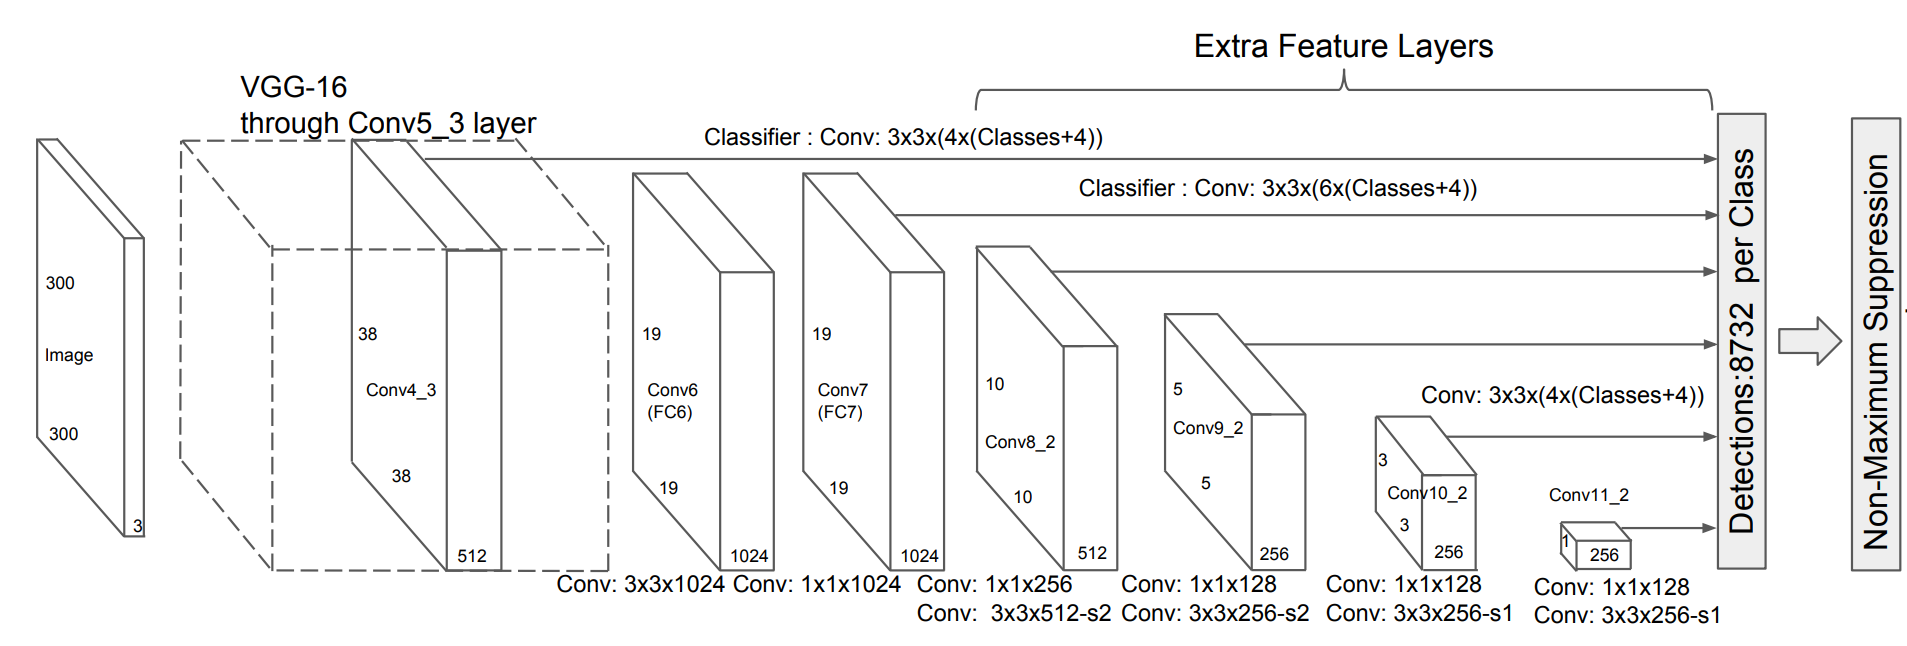
\includegraphics[width = 0.9\textwidth]{ssd.png}
    \caption{SSD算法框架}
    \label{ssd}
\end{figure}

最近几年基于 SSD 基础上的改进版本也很多,主要有 DSSD\cite{fu2017dssd}、
DSOD\cite{shen2017dsod}、FSSD\cite{li2017fssd}等。DSSD 主要针对 SSD 算法的浅层 feature map 语义信息不
够充分导致对小目标不够鲁棒的问题,提出了用 ResNet-101 和 Deconvolution 模
型,使用反卷积将特征图进行上采样与原始特征图进行融合,skip 连接使浅层
feature map 具有更好的表征能力。以前的目标检测算法都是先在开源的数据集上
进行预训练,然后再进行微调(fine-tuning),虽然 fine-tuning 可以加速获得最终模
型,但是获得的模型结构灵活性差,计算量也大。针对以上问题 DSOD 算法提
出一种不需要预训练模型的目标检测算法,网络可以从零开始训练,并且效果可
以和 fine-tuning 的模型媲美。DSOD 可以看作是 SSD+DenseNet 的结合,减少了
参数量。

\subsection{红外图像目标检测研究现状}
近年来随着红外成像技术的发展,红外目标检测任务也成为了重点研究的问
题之一。但红外图像往往会存在着对比度低、缺少目标纹理信息、信噪比低等特
点,使得红外目标检测任务增加了难度。因此如何攻克因红外图像特性带来的技
术难点,是未来红外目标检测的发展方向。
目前红外目标检测方法主要分为以下几种类别:基于目标的先验知识进行目
标检测、使用模板对目标进行匹配、基于机器学习方法进行目标检测等。

基于目标的先验知识进行目标检测的方法主要是用于红外场景简单并且目
标与背景之间对比度比较高的情况。此类方法往往需要人为的去建立一个数据库
作为先验知识,后续根据检测目标的特征与数据库进行比对。此种方法不但复杂
并且一旦检测其他的目标或检测环境发生变化时,就需要重新获取先验知识,因
此此类方法灵活性差,没有适用性。

使用模板对目标进行匹配的红外目标检测方法是利用统计的方法从之前的
数据中得到模板,然后将红外探测器获取到的红外图像与模板进行相似性度量,
根据二者相似度,从而实现对红外图像中的目标进行定位以及类别的确定\cite{宋曦2010一种基于模板匹配的目标识别方法}。

1997 年,Maes 等人提出了最大互信息图像匹配方法,相比传统算法减少了计算
量,之后广泛应用于目标检测等多个领域\cite{maes1997multimodality}。1999 年,Studholme C 等人考虑重
叠统计量作为重要因素,提出将梯度引入互信息中解决联合熵的不足,并针对互
信息不能提供有用的对齐措施问题将互信息进行归一化处理,实验结果显示能够
实现对目标的快速检测\cite{studholme1999overlap}。之后几年,Russakoff 等人提出互信息作为图片相似
性度量,没有考虑每个像素之间的关系,缺少空间信息。因此将空间信息引入到
互信息中进行扩展,提出了新的相似性度量方法-区域互信息\cite{russakoff2004image}。2005 年,顾静
良等人针对复杂背景下获得的红外图像具有大量的噪声并且存在弱小目标的情
况下,提出了一种适合红外弱小目标识别的相似性度量方法,并使用自适应模板
匹配方法来提高算法的稳定性\cite{顾静良2005基于自适应模板匹配的红外弱小目标检测}。2008 年,钟都都等人提出了一种改进的基于
模板匹配的跟踪算法,改良传统的模板匹配方法,用 SUSAN 算子提取目标的角
点特征,将特征信息和灰度信息进行加权融合来提取模板,所提出的算法用于红
外跟踪系统不仅能保证实时性,还具有稳定性和抗漂移能力\cite{钟都都2008用于红外目标跟踪的模板匹配改进算法}。虽然使用模板对
目标进行匹配的方法实现起来比较简单,但对模板的选择有很高的要求,同时如
果模板比较简单难以适用于复杂场景,如果将模板进行改进又会增加工作量,难
以适应各种场合以及目标的需要。因此目前该方法已逐渐被基于机器学习的方法
所替代,除了偶尔应用在简单场景下的工程项目外,几乎很少有应用。
基于机器学习的红外目标检测方法主要分为两类:一类是通过手工提取特征
对红外图像中感兴趣的区域(ROIs)进行提取最后使用分类器进行分类。主要分
为区域选择、特征提取和分类器分类三个步骤。之后还有基于目标特性进行 ROIs
区域搜索、阈值分割等方法。在深度学习出现之前,基于机器学习的红外目标
检测算法因其较强的鲁棒性,成为红外目标检测使用的主流算法。但由于该类算
法存在大量的计算冗余并且因为红外图像本身存在大量的噪声等特性,使得该算
法用于红外目标检测上的效果并不好。随着近年来深度学习的发展,卷积神经网
络强大的特征提取能力以及大数据处理能力,在可见光目标检测上取得了巨大的
成功。近几年也陆续出现了使用深度学习算法进行红外目标检测的研究。Aparna
Akula 等人为了开发一种隐私保护系统来实现自动识别人的行为,通过自建红外
数据集,并针对数据集设计目标检测网络,检测精度达到 87.44$\%$,验证了卷积
神经网络用于红外目标检测的可行性\cite{akula2018deep}。许来祥等人结合红外图像的特点,提出了一种基于 ZFNet 改进的目标检测网络,在 ZFNet 基础上加空间变换网络提高
鲁棒性,并深入讨论 Dropout 层设置参数不同带来的影响\cite{许来祥2020基于改进}。虽然目前基于深度
学习的红外目标检测识别的研究并不多,但之后随着开源红外数据集的增多,相
关的研究会越来越多。

\section{本文主要研究内容}
本文主要针对红外图像无人机目标检测任务存在的问题进行研究,在课题研究过程中,主要分析并研究了以下几个方面的问题:

(1)红外无人机数据匮乏

目前开源的红外数据比较少,而基于深度学习的目标检测网络需要有充足的
数据支撑,因此本文的研究内容包括了红外无人机目标数据集的标注和制作。

(2)红外图像的检测特点和难点

由于红外图像在获取的过程中主要受到红外探测器和环境噪声的影响以及
红外辐射原理所造成的红外图像质量差、信噪比低等不利于检测的缺点。因此在
网络输入图像之前对红外图像进行预处理提高图像信噪比、增大图像包含的信息量也是重点研究的内容。

(3)待测无人机目标的尺度变化

本文的任务是红外图像无人机目标检测,场景的特点是小目标的出现频率较高,因此算法对较小尺寸目标的检测能力也是本文的研究内容。

(4)无人机目标检测的定位问题

在 YOLOv5 中使用IoU作为损失函数,有可能产生定位不准的问题,因此本文重点研究了对YOLOv5网络目标框定位损失函数的改进。

(5)检测算法的嵌入式实现以及实时推理

在某些特殊应用场景中难以满足较高的计算能力,如在嵌入式设备上使用,
无法保证在速度较快的情况下实现高精度检测,这种时候就需要设计出适用于特
定任务下的轻量级实时目标检测网络,也是本课题重点研究的问题。

\section{本文组织结构}
本文以红外目标检测算法所存在的问题展开研究,研究了红外无人机检测并实现嵌入式应用。本文分为四个章节,每
个章节的主要内容如下:

第1章为绪论。首先介绍了基于深度学习的红外目标检测算法的研究背景和
意义,然后针对当前主流的目标检测算法的国内外研究发展现状做了发展脉络介
绍,介绍了红外目标检测算法在传统方向和深度学习方向的相关研究工作,最后
介绍了本文具体的研究内容和组织结构。

第2章介绍了红外目标检测相关理论和工作基础。首先介绍了卷积神经网络
的主要组成结构以及目标检测的评价指标,接着对红外图像如何获得的过程进行
了简单的介绍,最后介绍了红外图像的主要特征。

第3章主要介绍了建立红外无人机图像数据集的过程,研究了目前主流的图像预处理方法,并进行了测试,用以提高整
个图像的信息量,并提出了两种新的红外数据增强算法,并将该算法在数据集上
进行了测试和结果分析,此外还对YOLOv5网络的目标框定位损失函数进行了改进,并对改进后的算法进行了实验和分析。

第4章实现红外无人机检测的轻量化和实时嵌入式应用。由于实际项目需要完成对无
人机的实时检测,因此本文重点研究了算法的轻量化和嵌入式部署,将第三章中研究的较高精度的红外无人机检测算法通过轻量化方法实现精度和速度的平衡,然后将得到的新算法部署在嵌入式设备上,进行更加贴近红外无人机检测应用场景的功能测试,基本可以达到实时推理,验证本文研究算法的适用性。

